% !TEX program = xelatex

% Base
\documentclass{article}
\usepackage[a4paper,margin=1in]{geometry}

% Locale
\usepackage{polyglossia}
\setdefaultlanguage[localalph=true]{slovenian}
\usepackage[autostyle]{csquotes}
\DeclareQuoteAlias{german}{slovene}

% Bibliography
\usepackage[backend=biber,style=numeric]{biblatex}
\addbibresource{/home/martin/literatura.bib}

% Math
\usepackage{amsmath}
\usepackage{amssymb}
\usepackage{siunitx}

% Imported pdf_tex figures
\usepackage{graphicx,import}
\usepackage{subfig}
\usepackage{color}

% Hyperlinks
\usepackage{hyperref}
\usepackage[svgnames]{xcolor}

% Pgfplots
\usepackage{amssymb}

% Styling
\numberwithin{equation}{section}
\setlength{\skip\footins}{1.5cm}

% Differential
\newcommand{\diff}{\mathrm{d}}

% "Defined as" symbol
\usepackage{mathtools}
\newcommand{\das}{\vcentcolon=}
\newcommand{\asd}{=\vcentcolon}

\title{Elektrooptični pojav v feroelektričnem tekočem kristalu}

\author{Martin Šifrar}

\begin{document}

\maketitle

\section{Naloga}

\begin{enumerate}
    \item Pri konstantni napetosti spreminjajte frekvenco in pri vsaki frekvenci komponenti signala v fazi in iz faze.
    \item Narišite obe komponenti signala kot funkciji frekvence in s prilagajanjem komponent~(\ref{eq:re-im}) določite relaksacijski čas.
    \item Narišite tudi razmerje med signalom pri fazi $90^\circ$ in signalom pri fazi $0^\circ$ v odvisnosti od frekvence in s prilagajanjem določite relaksacijski čas.
\end{enumerate}

\begin{figure}[h]
    \begin{center}
        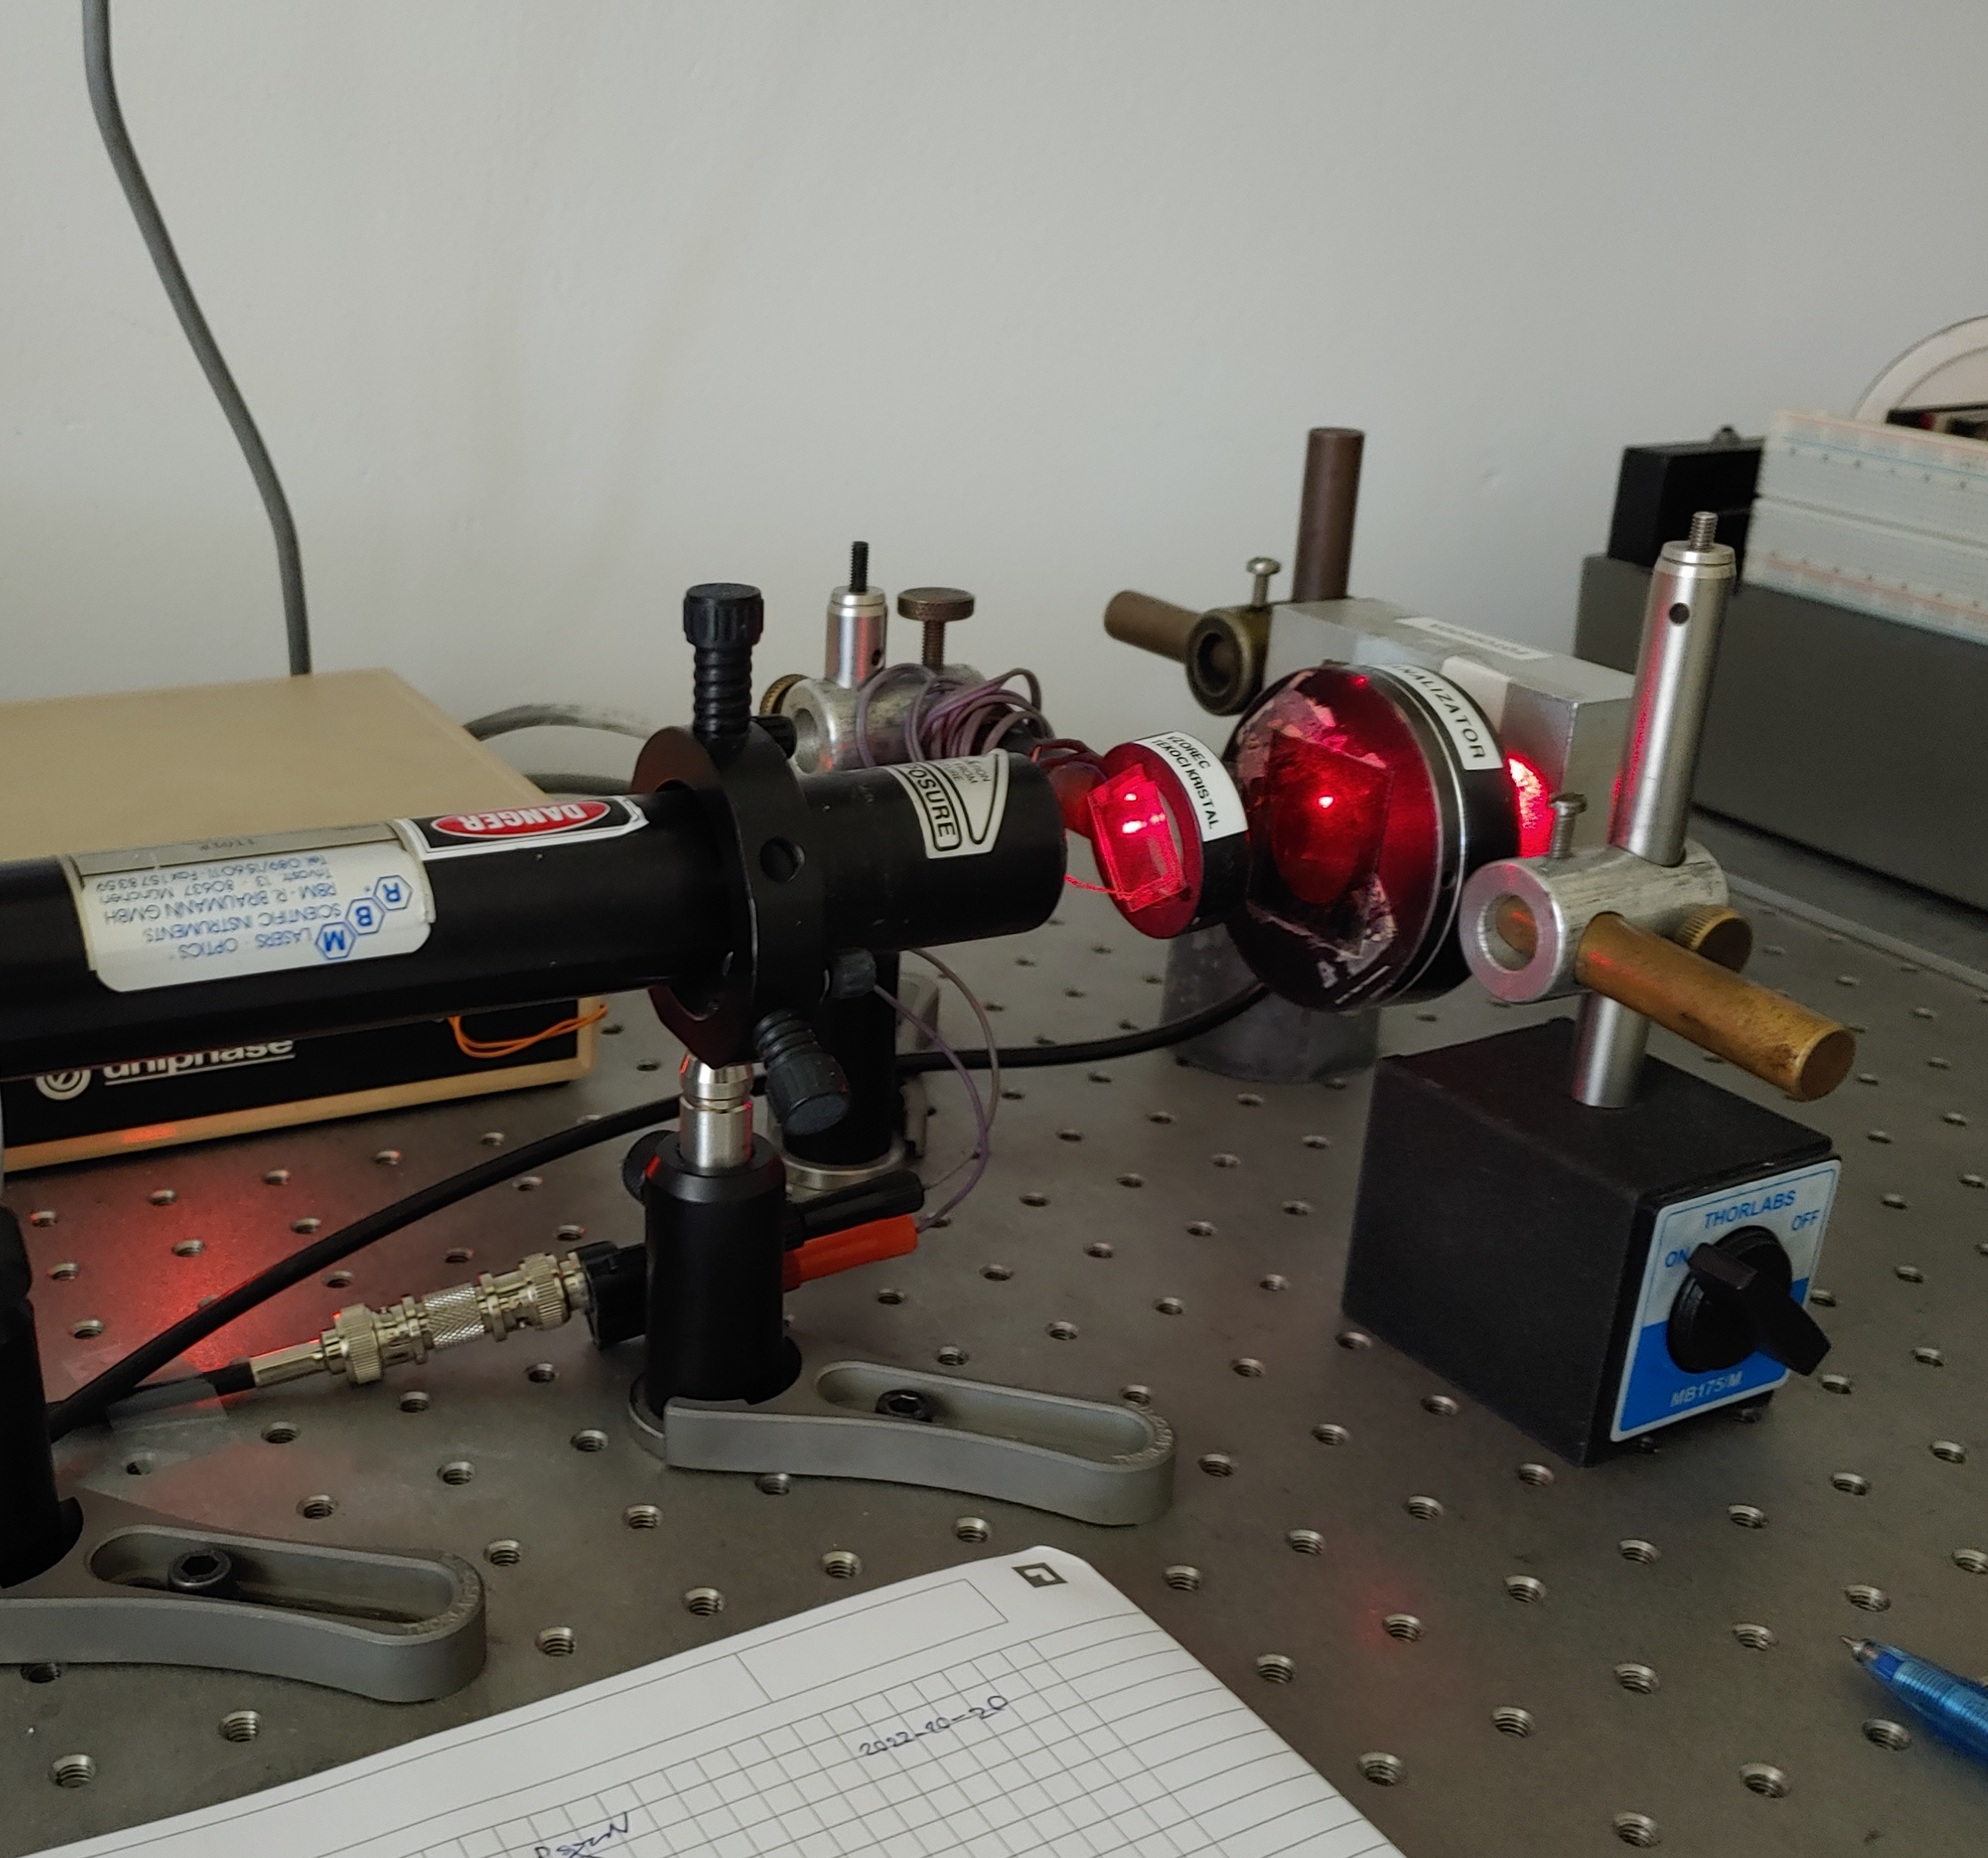
\includegraphics[width=0.6\textwidth]{setup.png}
    \end{center}
    \caption{Postavitev laserja, vzorca in analizatorja.}
    \label{fig:setup}
\end{figure}

\section{Meritve}

Prvo pri fiksni referenčni frekvenci

\begin{equation*}
    \nu_\mathrm{ref} = 30\,\mathrm{Hz}
\end{equation*}

pomerimo odziv polarizacije (sorazmerno napetosti na fotodiodi) v odvisnosti od modulacijske amplitude $U_0$~(slika~\ref{fig:modulation}).

\begin{figure}
    \begin{center}
    \includegraphics{modulation.pdf}
    \end{center}
    \caption{Odziv sorazmeren $|\delta P|$, tj. amplitudi napetosti na fotodiodi, v odvisnosti od modulacijske amplitude $U_0$. Prikazani del meritev je zelo blizu premici, za višje $U_0$ pa je odziv nelinearen. \textbf{Napake so premajhne, da bi se jih na grafu lepo videlo, povprečna relativna napake je približno $0.1\%$.}}
    \label{fig:modulation}
\end{figure}

Nato pri fiksni modulacijski amplitudi

\begin{equation*}
    U_0 = 0.4\,\mathrm{V}
\end{equation*}

pomerimo še odvisnost kompleksne napetosti, sorazmerne polarizacijskemu odzivu v kristalu. Meritve vidimo na sliki~\ref{fig:XY-by-freq}.

\begin{figure}
    \begin{center}
        \includegraphics{XY-by-freq.pdf}
    \end{center}
    \caption{Realni in kompleksni del napetosti, ki je sorazmerna odzivu $\delta P$ v kristalu. Frekvenčni odziv pri konstanti modulacijski amplitudi $U_0$. Prilagojene krivulje so oblike~(\ref{eq:re-im}).}
    \label{fig:XY-by-freq}
\end{figure}

Odziv polarizacije je po Debyjevem relaksacijskem modelu oblike

\begin{equation*}
    \delta P = \delta P_0 \frac{1}{1+i\omega\tau},
\end{equation*}

kar lahko po razcepu na realno in imaginarno komponento zapišemo kot

\begin{equation}
    \frac{\delta P}{\delta P_0} = \left\{ \frac{1}{1+\omega^2\tau^2} \right\} + i\left\{ \frac{-\omega\tau}{1 + \omega^2\tau^2} \right\}.
    \label{eq:re-im}
\end{equation}

kar lahko prilagodimo na naše meritve odziva. Prilagojene krivulje vidimo na sliki~\ref{fig:XY-by-freq}. Za $\tau$ dobimo dve precej različni vrednosti, vzamemo njuno sredinsko vrednost

\begin{equation*}
    \tau = (3.4 \pm 0.1)\,\mathrm{ms},
\end{equation*}

prav tako napravimo z amplitudo relaksacije (oz. napetostjo, ki ji je sorazmerna)

\begin{equation*}
    \delta P_0 = (134 \pm 0.2)\,\mathrm{mV}.
\end{equation*}

\begin{figure}
    \begin{center}
    \includegraphics{linearized.pdf}
    \end{center}
    \caption{Zdeljena oblika izraza~(\ref{eq:re-im}), ki je preprosto premica po krožni frekvenci $\omega$, z naklonom $\tau$. Predstavlja tangens faznega zamika polarizacije za modulacijskim poljem. Vidimo, da so napake za velike frekvence zelo velike, saj je tam relativna napaka imaginarne komponente $X$ velika.}
    \label{fig:linearized}
\end{figure}

Alternativno lahko v izrazu~\ref{eq:re-im} delimo imaginarno komponento z realno komponento. Če realno komponento onačimo $X$, imaginarno pa $Y$, velja

\begin{equation*}
    -Y/X = \tau\omega.
\end{equation*}

Na to linearizirano obliko prilagodimo premico, iz česar izračunamo

\begin{equation*}
    \tau = (2.3 \pm 0.2)\,\mathrm{ms}.
\end{equation*}

\end{document}
